\documentclass{beamer}
\usetheme{Boadilla}
\usepackage{ngerman}
\usepackage{graphicx}
\usepackage{amsmath}


\title{Skisockenwärmer}
\subtitle{Optimierung der Leistungsregelung}
\author{Laurin Weitzel}
\institute{Simulation mit pSpice}
\date{\today}

\begin{document}
	\begin{frame}
		\titlepage
	\end{frame}
	\begin{frame}
		\frametitle{Übersicht}
		\tableofcontents
	\end{frame}
	\section{Einleitung}
	\subsection{Problemstellung}
	\begin{frame}
		\frametitle{Problemstellung}
		\begin{columns}
			\column{0.5\textwidth}
			\begin{itemize}
				\item{Kalte Füße beim Skifahren}
				\begin{itemize}
					\item{Elektronisch beheizte Skisocken}
					\item{Integrierte Batterie}
				\end{itemize}
				\item{Verbrannte Füße beim Skifahren}
				\begin{itemize}
					\item{Leistungsregelung}
				\end{itemize}
				\item{Begrenzte Batteriekapazität}
				\begin{itemize}
					\item{Maximierung des Wirkungsgrades}
				\end{itemize}
			\end{itemize}
			\column{0.5\textwidth}
			\begin{figure}[tbh]
				\centering
				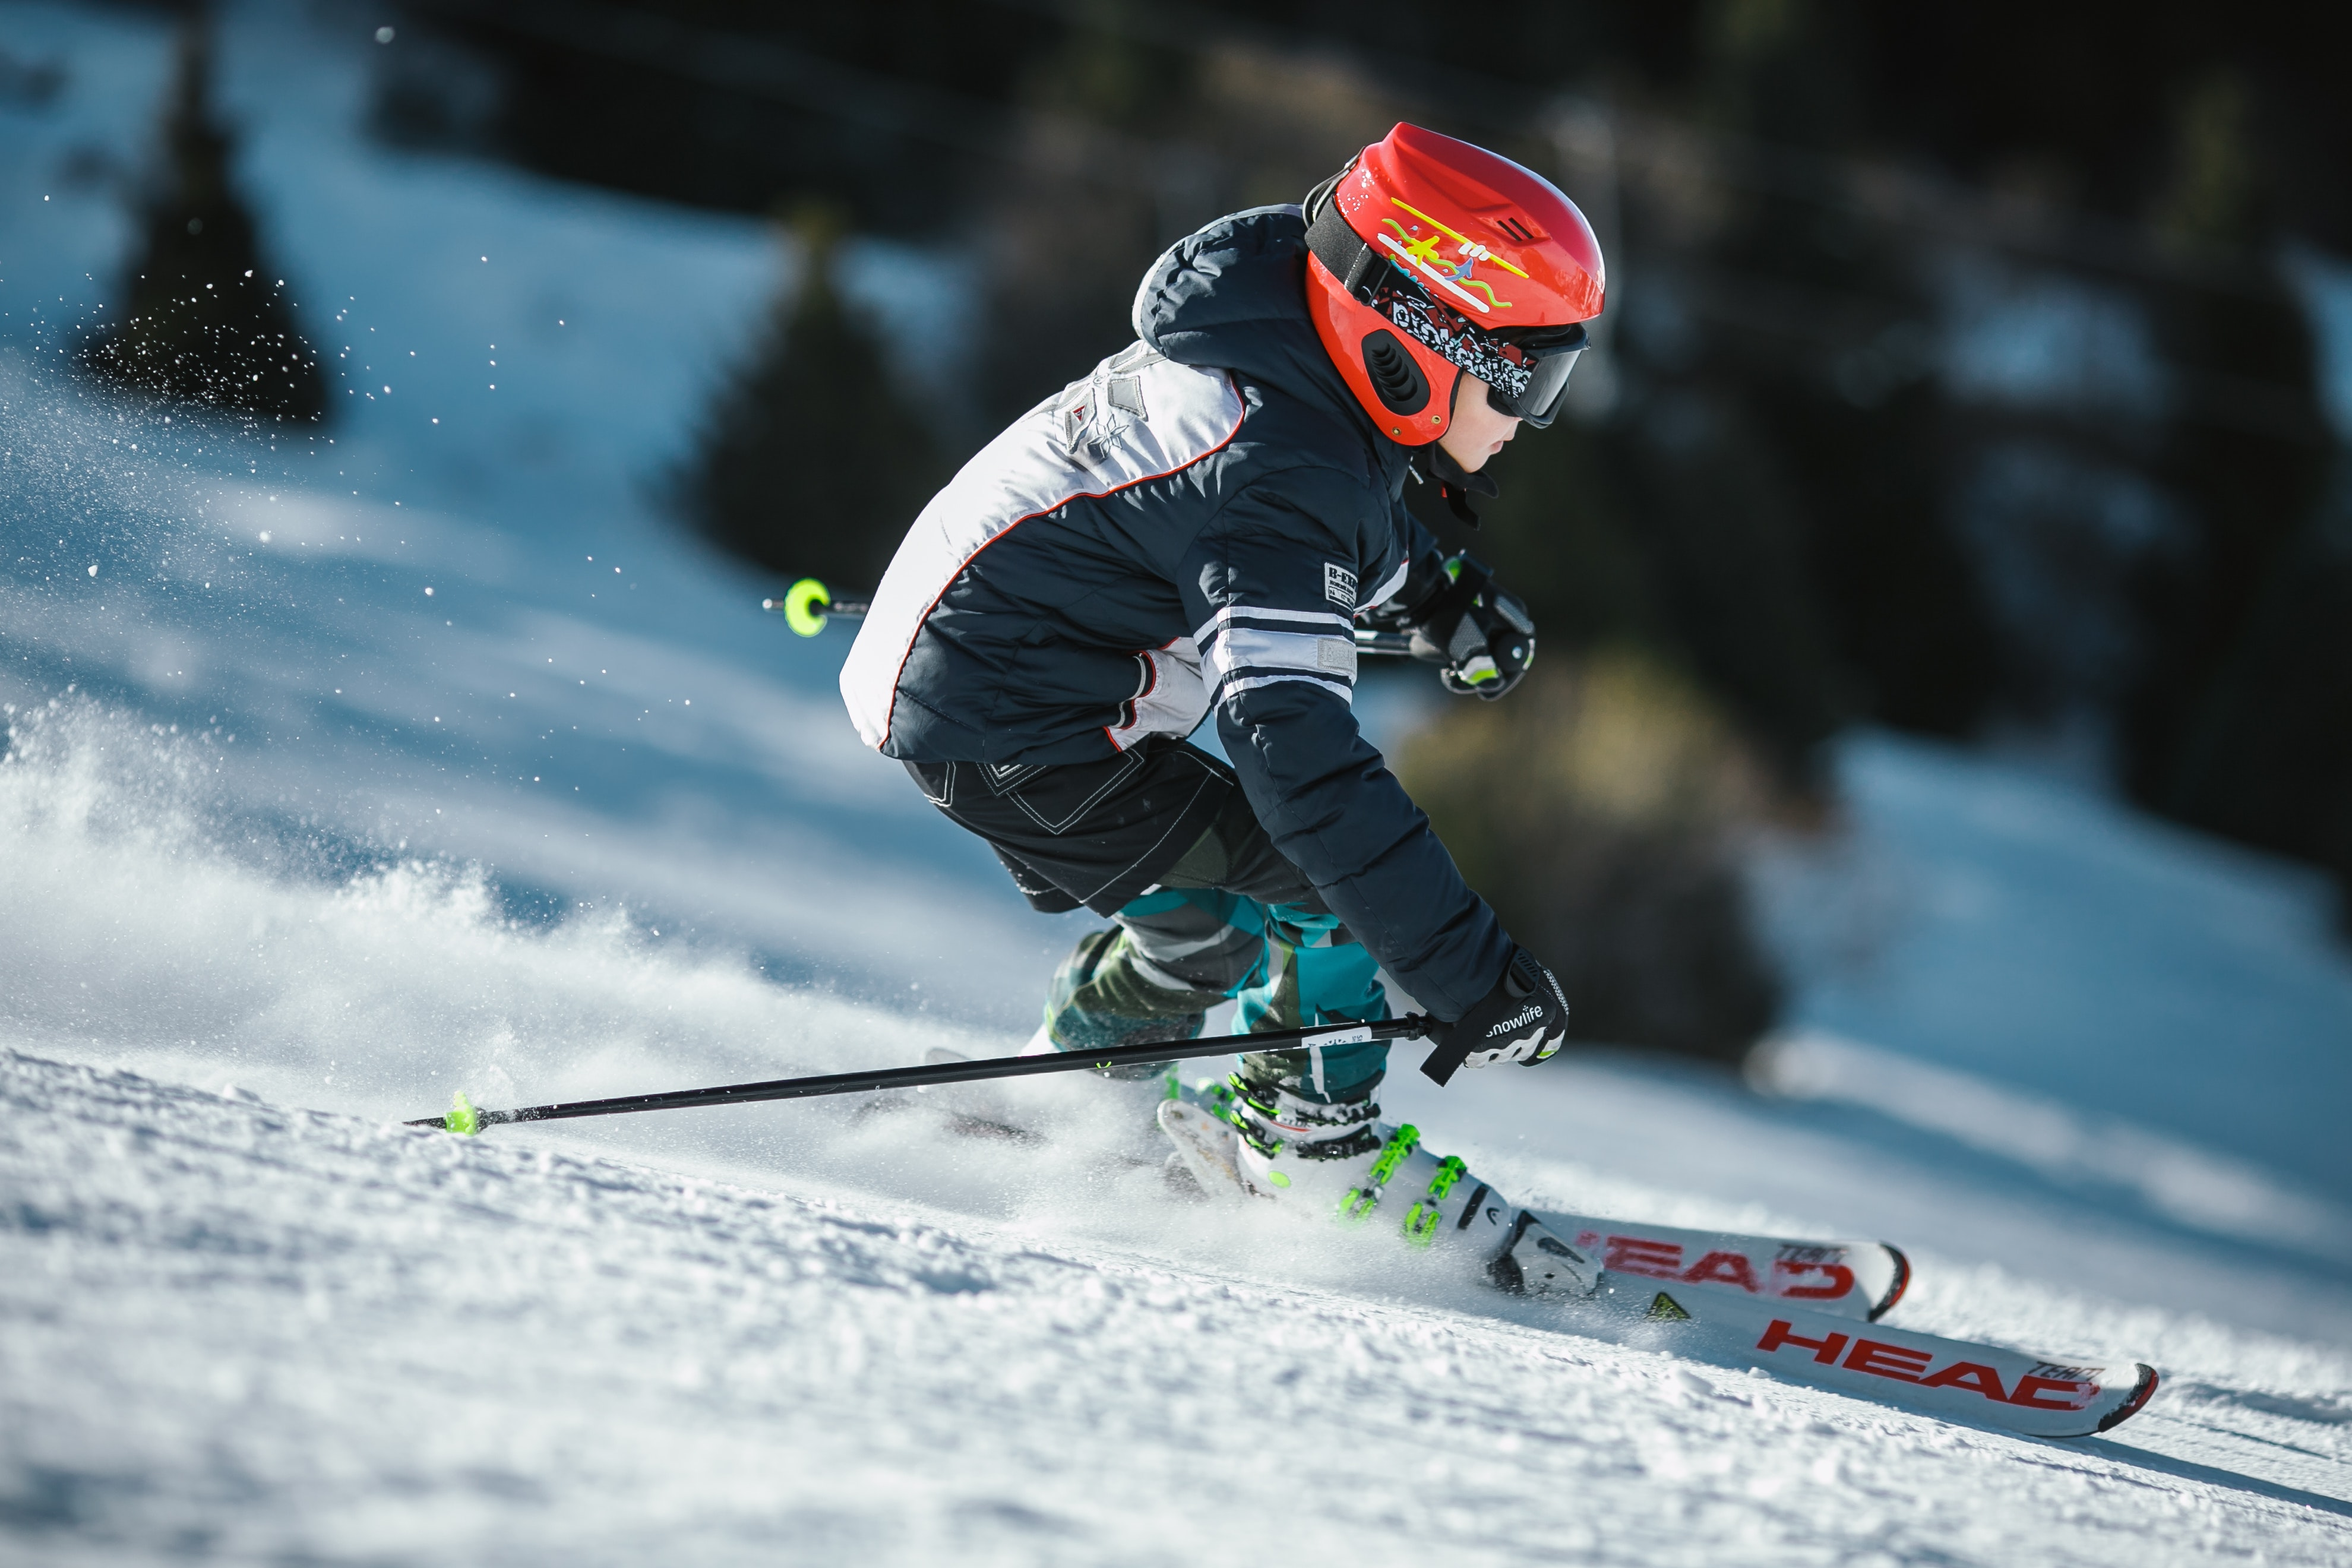
\includegraphics[width=1\linewidth]{medien/skifahrer}
				\caption[Nicht ich auf Skiern.]{Definitiv nicht ich. Zur Verfügung gestellt von: www.pexels.com/de-de/@visitalmaty/}
				\label{fig:skifahrer}
			\end{figure}
		\end{columns}
	\end{frame}
	\subsection{Optimierungsparameter}
	\begin{frame}
		\frametitle{Optimierungsparameter}
		\begin{itemize}
			\item{Kosten}
			\begin{itemize}
				\item{Leistungselektronik}
				\item{Batterie}
				\begin{itemize}
					\item{Optimierung des Wirkungsgrades}
				\end{itemize}
			\end{itemize}
			\item{Nutzerfreundlichkeit}
			\begin{itemize}
				\item{Batterie soll den ganzen Tag lang halten}
				\item{Regelung möglichst einfach gestalten}
			\end{itemize}
		\end{itemize}
	\end{frame}
	\section{Lösungsansätze}
	\subsection{Widerstandsregler}
	\begin{frame}
		\frametitle{Widerstandsregler}
		\begin{columns}
			\column{0.5\textwidth}
			\begin{figure}[tbh]
				\centering
				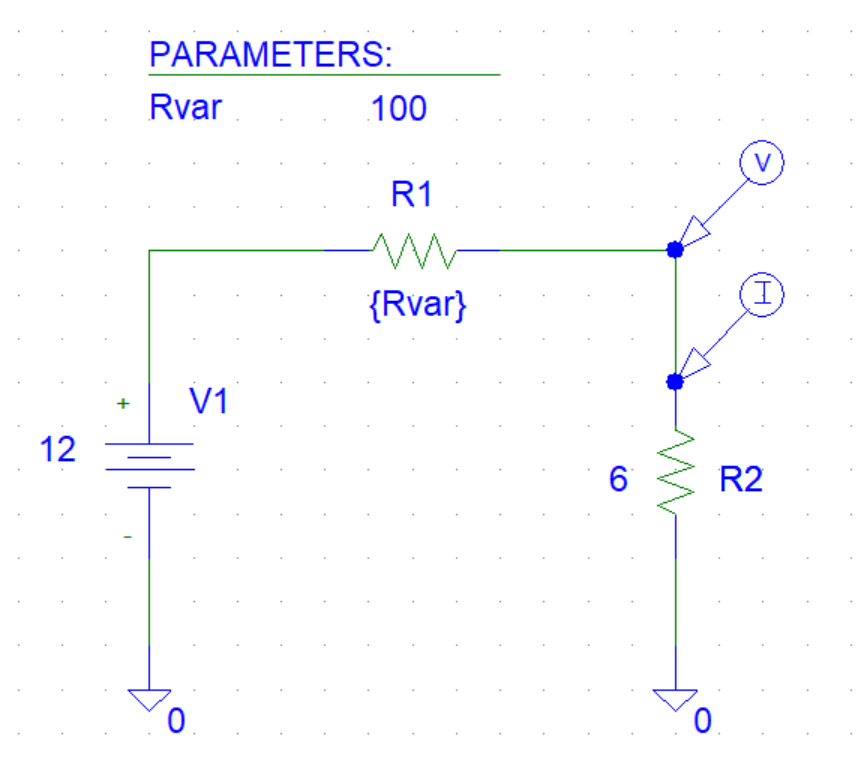
\includegraphics[width=1\linewidth]{medien/V1-0}
				\caption[Erster Aufbau]{Aufbau eines einfachen Spannungsteilers als Leistungsregelung.}
				\label{fig:aufbau1}
			\end{figure}
			\column{0.5\textwidth}
			\begin{itemize}
				\item{Einfache Leistungsanpassung}
				\begin{itemize}
					\item{z.B. durch Potentiometer}
					\item{Keine zusätzlichen Bauteile}
				\end{itemize}
				\item{Schlechter Wirkungsgrad}
				\begin{itemize}
					\item{Viel Leistung an R1}
				\end{itemize}
			\end{itemize}
		\end{columns}
	\end{frame}
	\begin{frame}
		\frametitle{Widerstandsregler}
		\begin{columns}
			\column{0.5\textwidth}
			\begin{figure}[tbh]
				\centering
				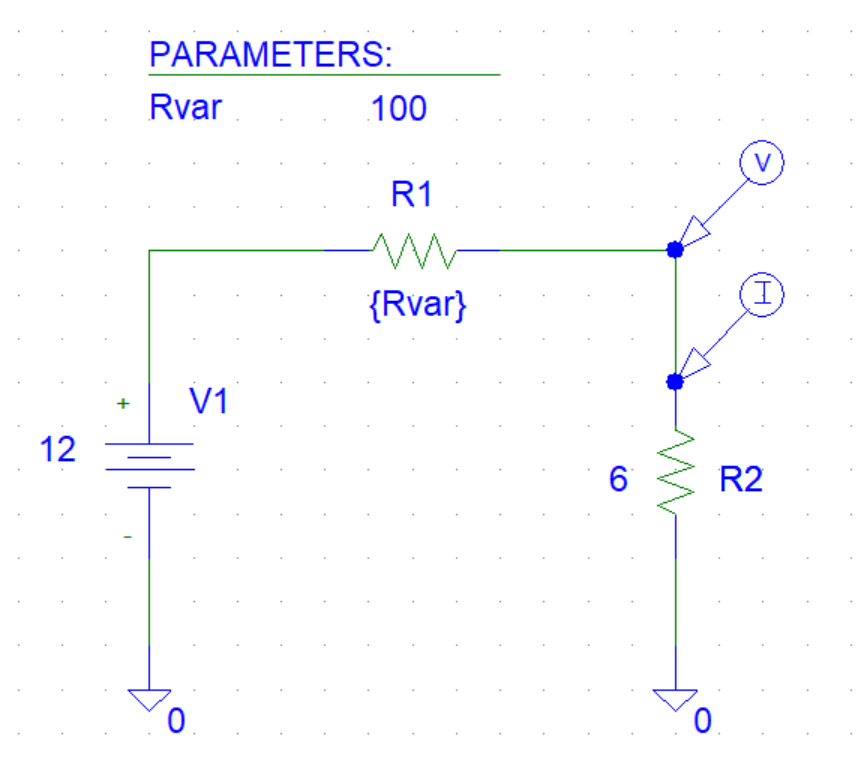
\includegraphics[width=1\linewidth]{medien/V1-0}
				\caption[Erster Aufbau]{Aufbau eines einfachen Spannungsteilers als Leistungsregelung.}
			\end{figure}
			\column{0.5\textwidth}
			\begin{align*}
				R_{ges}&=R_1+6\,\Omega \\
				I_{ges}&=\frac{12\, V}{R_{ges}} \\
				P_{heiz}=I_{ges}^2R_2&=12\, V\frac{6\,\Omega}{\left( R_1 + 6\,\Omega\right) ^2} \\
				P_{verlust}=I_{ges}^2R_1&=12\, V\frac{R_1}{\left( R_1 + 6\,\Omega\right) ^2} \\
				\theta &= \frac{P_{heiz}}{P_{heiz}+P_{verlust}}
			\end{align*}
		\end{columns}
	\end{frame}
	\subsection{Operationsverstärker}
	\begin{frame}
		\frametitle{Operationsverstärker}
	\end{frame}
	\subsection{Verbesserungsvorschlag}
	\begin{frame}
		\frametitle{Verbesserungsvorschlag}
	\end{frame}
	\section{Auswertung}
	\subsection{Vergleich der Ansätze}
	\begin{frame}
		\frametitle{Vergleich der Ansätze}
	\end{frame}
	\subsection{Fazit}
	\begin{frame}
		\frametitle{Fazit}
	\end{frame}
\end{document}